\documentclass[aps,pnas,float]{revtex4}
\usepackage{amsmath,bm,epsfig}
%\topmargin=.2in
\textheight=9.0in
\newcommand{\cor}{\rm cor}
\newcommand{\ph}{\rm ph}
\newcommand{\rel}{\rm rel}
\newcommand{\M}{{\rm M}}
\newcommand{\e}{{\rm e}}
\newcommand{\ud}{\mathrm{d}}
\renewcommand{\k}{{\bf k}}
\newcommand{\wt}[1]{\widetilde{#1}}
\newcommand{\B}[1]{{\bm{#1}}}%% Bold Roman & Greek Lower & Upper Case
\newcommand{\C}[1]{{\mathcal{#1}}}    %%   Calligrapfic Upper case
%\usepackage[dvips]{color}
%\usepackage[notcite,notref]{tshowkeys}

\begin{document}

\title{Supplementary information for: shear bands as manifestation of a criticality in yielding amorphous solids}

\author{Giorgio Parisi$^1$, Itamar Procaccia$^2$, Corrado Rainone$^2$ and Murari Singh$^2$ }
\affiliation{$^1$Dipartimento di Fisica, Sapienza Universit\'a di Roma, INFN, Sezione di Roma I, IPFC -- CNR, Piazzale Aldo Moro 2, I-00185 Roma, Italy\\$^2$Department of Chemical Physics, the Weizmann Institute of Science, Rehovot 76100, Israel}
\maketitle

\section{The longitudinal correlation function}

Let us start from the expression of the free energy of a glass state, prepared by equilibrating a generic glass former down to a glass transition temperature $T_g$ where it can still be equilibrated, and then quenching it out of equilibrium to a given temperature $T<T_g$. Such a free energy was first defined in~\cite{FP95} in the context of spin-glass physics. Its definition in the case of structural glasses, and its computation in the particular case of hard spheres were first discussed in~\cite{RUYZ15}. The definition, in the case of a generic glass former made of $N$ particles is based on comparing two configurations $X^a$ and $X^b$ of the same glass. Here
\begin{equation}
X^a \equiv \{\B r_i^a\}_{i=1}^N \ , \quad X^b \equiv \{\B r^b_i\}_{i=1}^N \ ,
\end{equation}
where the labeling $\B r_i$ refers to the position of the same particle $i$ in the two different configurations.
For a generic interaction potential $V(X)$ the definition of the free energy is
\begin{equation}
f[T,T_g] \equiv -\frac{1}{\beta N} \int dX_0\ \frac{e^{-\beta_g V(X_0)}}{Z_g}\ \log\left[\int dX_1\ e^{\beta V(X_1)}\delta(q^*_r - Q_{01})\right].
\label{eq:FP}
\end{equation}
where $\beta_g=1/(k_B T_g)$, $\beta=1/(k_B T)$ and $q^*_r$ is the value of $q_r \neq 0$ whereupon the free energy attains a local minimum~\cite{RUYZ15}.
The overlap function $Q_{01}$ for any two configuration, say $a$ and $b$ is~\cite{JPRS16}
\begin{equation}
 Q_{ab} = \frac{1}{N}\sum_{i=1}^N \theta(\ell-|\boldsymbol{r}^a_i - \boldsymbol{r}^b_i|).
\end{equation}
Here $\ell$ is a coarse graining parameter (in~\cite{JPRS16}, $\ell
\simeq 0.3$ in Lennard-Jones units).
The idea is to consider the free energy at temperature $T$ of the glass former, which is \emph{constrained} to stay close to an amorphous configuration $X_0$ which is selected from the equilibrium ensemble, using the canonical distribution when the glass is still at equilibrium at $T_g$.

The properties and computation of the free energy \eqref{eq:FP} are discussed extensively in~\cite{RUYZ15,RU16}, so we refer the interested reader to those works. The explicit analytic computation is accomplished in the
mean field approximation. In our paper we use the results far from the mean field limit, but we ascertain that the relevant correlation functions that are fleshed out in the mean field calculation are the relevant ones also in the general case. Of course, critical exponents can differ. In the sequel we sketch how from this mean-field theory in terms of an overlap order parameter $Q_{ab}$ one can extract the definitions of the correlation functions that are expected to show critical behavior.

The outermost integral in the Eq.~\eqref{eq:FP} can be computed with the replica trick,
\begin{equation}
 f[T,T_g] = \lim_{s\to 0} \partial_s \Phi[T,T_g;s],
\end{equation}
where $\Phi$ is defined as
\begin{equation}
 \Phi[T,T_g;s] =  -\frac{1}{\beta N}\log \int dX_0\ dX_1 \cdots dX_s e^{-\beta_g V(X_0)} e^{- \beta V(X_1)}\delta(q-Q_{01})\cdots e^{- \beta V(X^s)}\delta(q-Q_{0s}),
\end{equation}
so we are considering $s$ replicas of the $X$ configuration. In infinite dimensions for the case of hard spheres it was shown~\cite{KPZ12} that the functional defined above can be written as
\begin{equation}
 \Phi = -\frac{1}{\beta N} \int \mathcal{D} Q_{ab}\ e^{-d S(Q_{ab})} \ .
\end{equation}
Here $\mathcal{D}Q_{ab}$ denotes an integration measure over all the distinct $Q_{ab}$s,
\begin{equation}
 \mathcal{D}Q_{ab} \equiv \prod_{a<b}^{0,s} dQ_{ab},
\end{equation}
and $d$ is the number of spatial dimensions. The functional $S(Q_{ab})$ is referred to as the ``replica action". In the mean-field limit $d\to\infty$, the integral above can be computed via the saddle point method~\cite{BenderAdvancedMethods}, which means that one must consider the optimum points in $Q_{ab}$ of the replica action $S(Q_{ab})$. This means that $S(Q_{ab})$ plays the role of a \emph{Gibbs free energy}, i.e. the free energy for fixed order parameter. An illustrative example is the case of a Curie-Weiss model (mean-field ferromagnet) wherein, for the Helmholtz free energy $F$ in zero magnetic field, one has~\cite{replicanotes}
\begin{equation}
 F(h=0,T) = \min_{m}G(m,T)
\end{equation}
where $G(m,T)$ is indeed the Gibbs free energy for fixed magnetization $m$. The minimization equation for $G$ is then the celebrated equation for the spontaneous magnetization
\begin{equation}
 \frac{\partial G}{\partial m} = 0 \Longrightarrow m = \tanh(\beta m)
\end{equation}
and the ferromagnetic phase transition takes place when the paramagnetic, $m=0$ minimum of $G$ flattens and splits in two degenerate minima with $m\neq 0$, which implies that at the critical temperature $\frac{\partial^2 G}{\partial m^2} = 0$. The derivation of the $S(Q_{ab})$ action in the case of mean-field hard spheres can be found in~\cite{KPZ12}.

In the present case the $f[T,T_g]$ plays the role of the Helmholtz free energy $F$ and the $S(Q_{ab})$ of the Gibbs free energy $G$. With this analogy, one can understand how the critical properties of glass states are related to the matrix of second derivatives of the replica action $S(Q_{ab})$,
\begin{equation}
 M_{ab;cd} \equiv \frac{\partial^2 S}{\partial Q_{a<b}\partial Q_{c<d}},\qquad a,b,c,d \in [1,s]
\end{equation}
in the limit $s \to 0$ (we stress that $X_0$ is not involved in this definition). The inverse $G_{ab;cd}$ of the tensor $M$, defined as
\begin{equation}
\sum_{e\neq f} M_{ab;ef}G_{ef;cd} = \frac{\delta_{ac}\delta_{bd} + \delta_{ad}\delta_{bc}}{2}
\end{equation}
is then the covariance matrix of the mean field theory
\begin{equation}
 G_{ab;cd} = \overline{\left<(Q_{ab}-\left<Q_{ab}\right>)(Q_{cd}-\left<Q_{cd}\right>)\right>},
\end{equation}
wherein the angled brackets denote the thermal average restricted to a single glass sample at temperature $T$ (that is over the canonical distribution of the $X_1$ configuration in the \eqref{eq:FP}), and the overbar denotes the average over all possible glass samples selected at $T_g$ (that is over the canonical distribution of the $X_0$ configuration in the \eqref{eq:FP}). This covariance tensor encodes the critical fluctuations of the system near the critical points whereupon the tensor $M_{ab;cd}$ develops a zero mode.

Let us now assume that the glass state under study is a single minimum of the free-energy landscape of the system wherein all replicas from $1$ to $s$ can move ergodically, this means that the replicas are all equivalent and the matrix $Q_{ab}$ must then be invariant by any replica permutation, an hypothesis referred so as replica-symmetric (RS).\\
In~\cite{RUYZ15} it is discussed how this is not true in all cases, i.e. there exist a regime wherein the glass basin undergoes an ergodicity breaking and fractures into sub-basins. Nevertheless, here we stick to the simple RS ansatz. In this case, since the action $S(Q_{ab})$ must in turn be invariant for any replica permutations, the most general form that the Hessian $M$ can take is
\begin{equation}
 M_{ab;cd} = M_1 \left(\frac{\delta_{ac}\delta_{bd} + \delta_{ad}\delta_{bc}}{2}\right) + M_2 \left(\frac{\delta_{ac} +\delta_{bd} + \delta_{ad} +\delta_{bc}}{4}\right) + M_3,
\end{equation}
and the same goes for the covariance matrix $G_{ab;cd}$. This form is completely general as it only pertains to the RS symmetry; then the only model-dependence is in the parameters $M_1$, $M_2$ and $M_3$, which must be computed case by case and are generally dependent on the external parameters like temperature or magnetic field.
The diagonalization of the tensor $M_{ab;cd}$ is an exercise of standard linear algebra and has been already carried out many times, see for example~\cite{CS92,BM79,DK98} and~\cite{Z10} where it is proposed as an exercise. It is found that the tensor $M$ has only three distinct eigenvalues
\begin{eqnarray}
 \lambda_R &=& M_1\\
 \lambda_L &=& M_1 + (s-1)(M_2+sM_3)\\
 \lambda_A &=& M_1 + \frac{s-2}{2}M_2,
\end{eqnarray}
and the same goes for the tensor $G$. Those three eigenvalues (or modes) are called the \emph{replicon}, \emph{longitudinal}, and \emph{anomalous}, respectively~\cite{Z10}.
We are interested in the longitudinal mode (which in the limit $s\to 0$ is degenerate with the anomalous one), which becomes soft at the yielding transition~\cite{RU16,UZ16}. Let us consider the $G$ tensor. Because of replica symmetry, there are only three distinct correlators that one can define, namely
\begin{eqnarray}
 G_{12;12} &=& \frac{G_1}{2} + \frac{G_2}{2} + G_3\\
 G_{12;13} &=& \frac{G_2}{4} + G_3\\
 G_{12;34} &=& G_3
\end{eqnarray}
and in the limit $s\to0$ we know that
\begin{equation}
 \frac{1}{\lambda_L} = G_1-G_2.
\end{equation}
It is then immediate to check that
\begin{eqnarray}
 G_{12;12} -2G_{12;13} + G_{12;34} &=& \frac{G_1}{2} \propto \frac{1}{\lambda_R} \equiv G_R\\
 G_{12;12} -4G_{12;13} + 3G_{12;34} &=& \frac{G_1-G_2}{2} \propto \frac{1}{\lambda_L} \equiv G_L
\end{eqnarray}
which then implies
\begin{equation}
 G_L(\boldsymbol{r}) = 2G_R(\boldsymbol{r}) -\Gamma_2(\boldsymbol{r}),
\end{equation}
with the definitions
\begin{eqnarray}
 G_R(\boldsymbol{r}) &\equiv& \overline{{\left<Q_{ab}(r)Q_{ab}(0)\right>}} - 2\overline{{\left<Q_{ab}(r)Q_{ac}(0)\right>}} + \overline{{\left<Q_{ab}(r)\right>\left<Q_{cd}(0)\right>}} \label{eq:defGR}\\
 \Gamma_2(\boldsymbol{r}) &\equiv& \overline{{\left<Q_{ab}(\boldsymbol{r})Q_{ab}(0)\right>}} -\overline{{\left<Q_{ab}(\boldsymbol{r})\right>\left<Q_{ab}(0)\right>}}, \label{eq:defG2}
\end{eqnarray}
as in the main text. We have used $\Gamma_2 = G_{12;12} - G_{12;34}$ which derives from replica symmetry, as $\left<Q_{12}\right>\left<Q_{12}\right> = \left<Q_{12}Q_{34}\right>$ in the replica-symmetric phase.

Let us now detail how to transform these definitions into quantities that can be measured in simulation. We start by "localizing" the definition of the $Q_{ab}$ overlap in the following way
 \begin{equation}
  Q_{ab}(\B r) \equiv \sum_{i=1}^N\theta(\ell-|\B r_i^a-\B r_i^b|)\delta (\B r -\B r_i^a).
  \label{eq:defQr}
 \end{equation}
 In a thermal simulation the $a$ and $b$ configurations would depend on the time $t$, and so would the $Q_{ab}(r)$, so one would need to perform the in-state thermal average $\left<\bullet\right>$ by considering the equilibrium value of these quantities. In the present paper we focus un athermal solids under quasi-static shear, so we do not have dynamics and the $a$ and $b$ configurations will simply be two distinct minima of the inter-particle potential obtained through the protocol described in the main text, and the thermal average will be the average over this ensemble of configurations which make up a glassy patch.\\
We now apply the definition \eqref{eq:defQr} in the \eqref{eq:defGR}, \eqref{eq:defG2} to construct the correlators. For illustrative purposes we use the $\Gamma_2(\boldsymbol{r})$. We get, omitting the overline to lighten the notation,
\begin{equation}
 \left<(Q_{ab}(\boldsymbol{x})-\left<Q_{ab}(\boldsymbol{x})\right>)(Q_{ab}(\boldsymbol{x}+\boldsymbol{r})-\left<Q_{ab}(\boldsymbol{x}+\boldsymbol{r})\right>)\right> = \sum_{ij}[(u^{ab}_i  -Q_{ab}) (u^{ab}_j - Q_{ab})]\delta (\B r + \boldsymbol{x} -\B r_i^a)\delta (\B x -\B r_j^a),
\end{equation}
with
 \begin{equation}
 u^{ab}_i \equiv \theta(\ell-|\boldsymbol{r}_i^a-\boldsymbol{r}_i^b|),
 \end{equation}
 as in the main text, and we used that $\left<Q_{ab}(x)\right> = Q_{ab}$. Because of translational invariance, the correlator is actually independent of $\boldsymbol{x}$. We can get rid of $\boldsymbol{x}$ by performing an integration over this variable, which, using the $\delta$-functions, gives as a result
\begin{equation}
\sum_{ij}[(u^{ab}_i  -Q_{ab}) (u^{ab}_j - Q_{ab})]\delta (\B r - (\B r_i^a- \boldsymbol{r}_j^a))
\end{equation}
then, following~\cite{BCJPSZ16}, we omit the terms with $i=j$ (which are anyway relevant only for $\boldsymbol{r} = 0$) and we normalize the correlator with the pair distribution function of the glass; we finally obtain
\begin{equation}
\frac{ \sum_{i\neq j}(u^{ab}_i-Q_{ab}) (u^{ab}_j-Q_{ab})\delta(\boldsymbol{r}-(\boldsymbol{r}_{i}^a-\boldsymbol{r}_{j}^a)) }{ \sum_{i\neq j}\delta(\boldsymbol{r}-(\boldsymbol{r}_{i}^a-\boldsymbol{r}_{j}^a)) } \equiv \tilde \Gamma_2(\B r),
\end{equation}
as in the main text. The derivation for the $\tilde G_R(\boldsymbol{x})$ is then an obvious generalization.




\section{Additional numerical results}

In the paper we have exhibited in Fig. 1 the susceptibilities $\chi_{_{G_R}}$ and $\chi_{_{\Gamma_2}}$. For
completeness we show here also the susceptibility $\chi_{_{G_L}}$, see Fig.~\ref{GL}.
As discussed in the paper, this susceptibility is very close to 2$\chi_{_{G_R}}$. On the other hand
the correlation functions themselves differ $G_R(x,y)$ and $G_L(x,y)$ differ significantly since
the function $\Gamma_2(x,y)$ is not positive definite, becoming negative towards the edges of the
available fields. This is seen clearly in Fig.~\ref{correlations} where we show the three
correlation function at the value of $\gamma=0.09405$.
%%%%%%%%%%%%%%%%%%%%%%%%%%%%%%%%%%%%%%%%%%%%%%%%%%%%%%%%%%%%%%%%%%%%%%
\begin{figure}[htpb]
 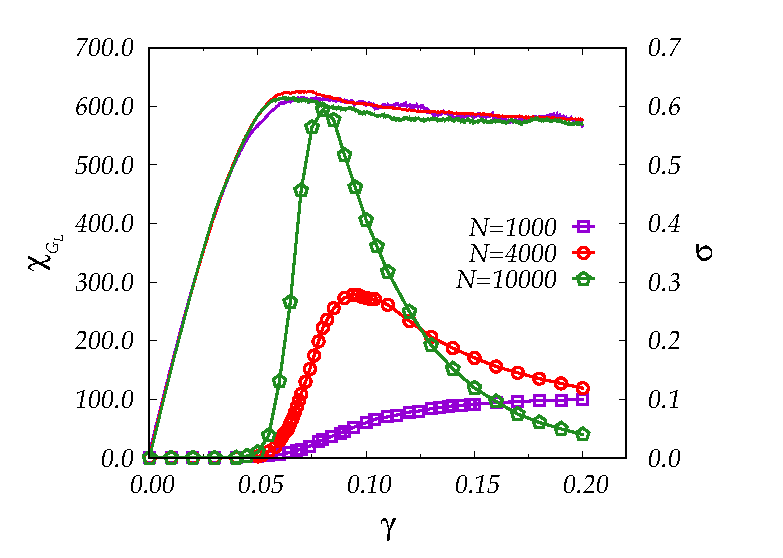
\includegraphics[width=0.5\textwidth]{spinodalSIFig1.eps}
 \caption{The susceptibility $\chi_{_{G_L}}$  as a function of $\gamma$ for the three systems sizes available. Superimposed are the stress vs. strain curves for comparison.
 The color code is violet for $N=1000$, red for 4000 and green for 10000.}  \label{GL}
\end{figure}
%%%%%%%%%%%%%%%%%%%%%%%%%%%%%%%%%%%%%%%%%%%%%%%%%%%%%%%%%%%%
%%%%%%%%%%%%%%%%%%%%%%%%%%
\begin{figure}[htpb]
 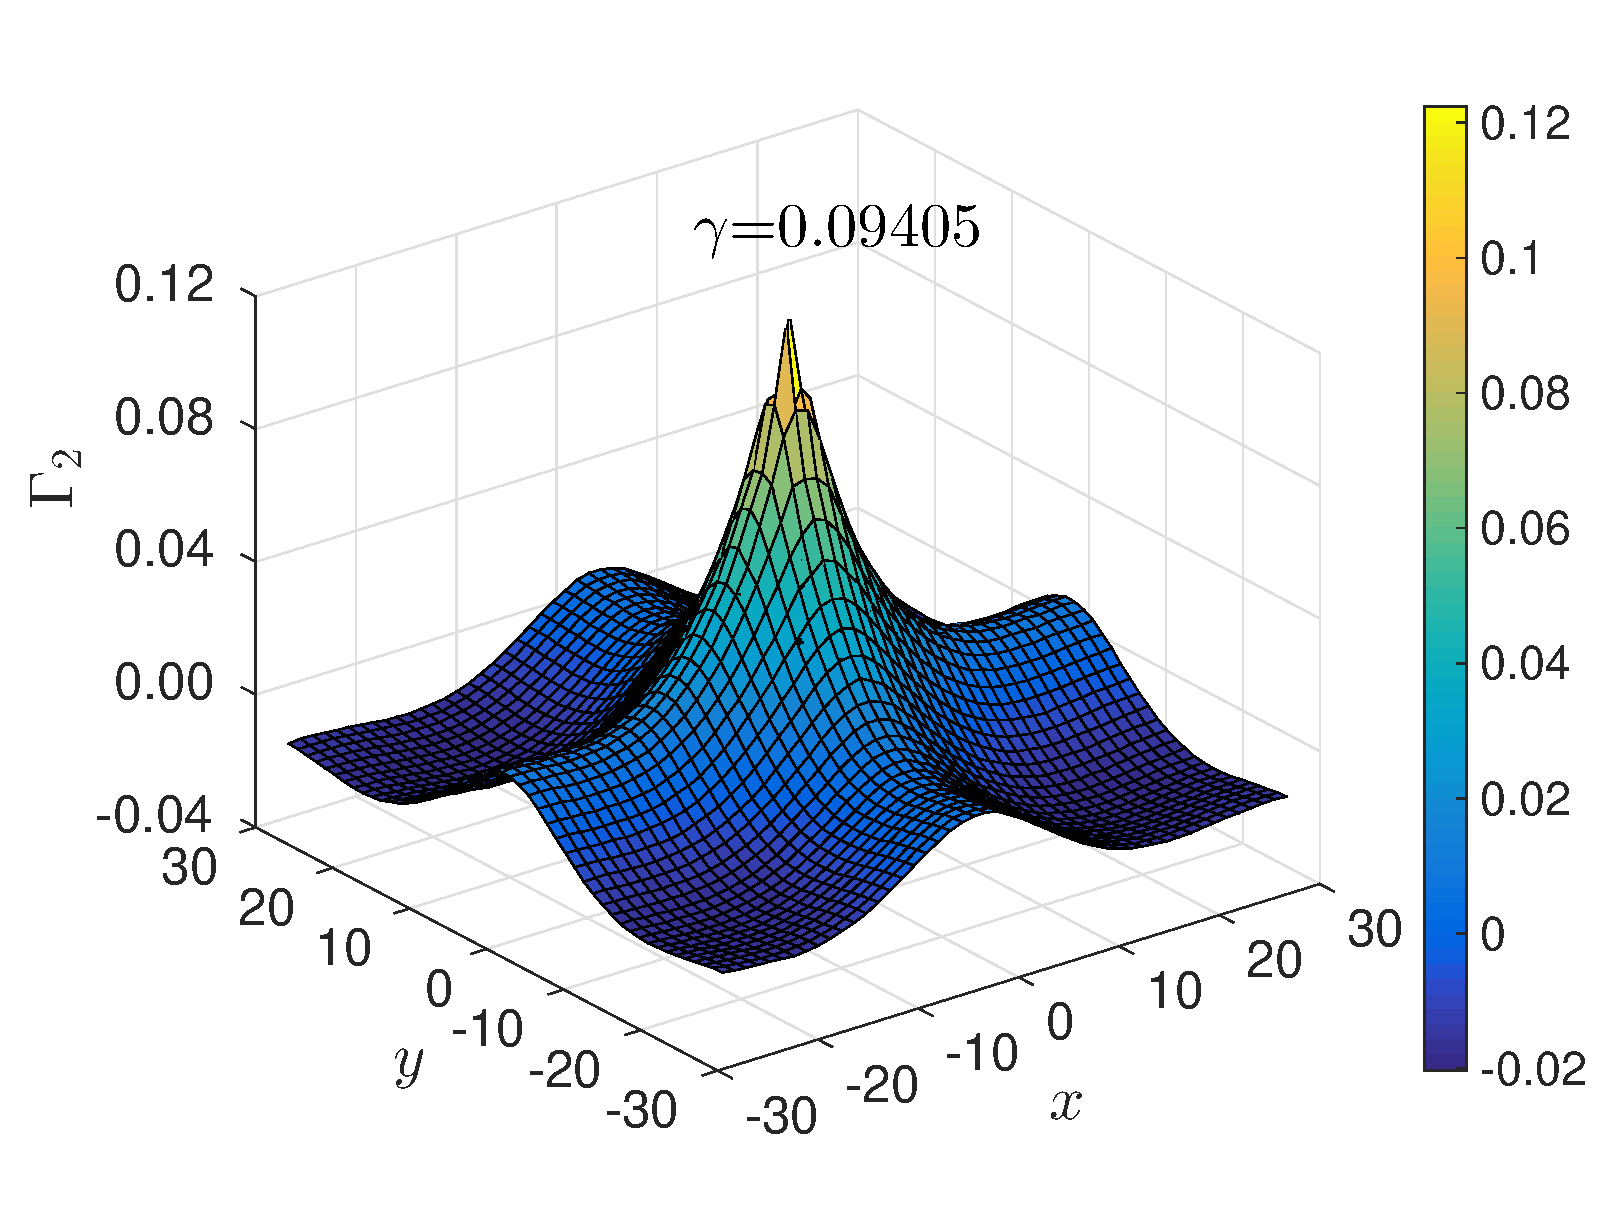
\includegraphics[width=0.3\textwidth]{spinodalSIFig2a.eps}
 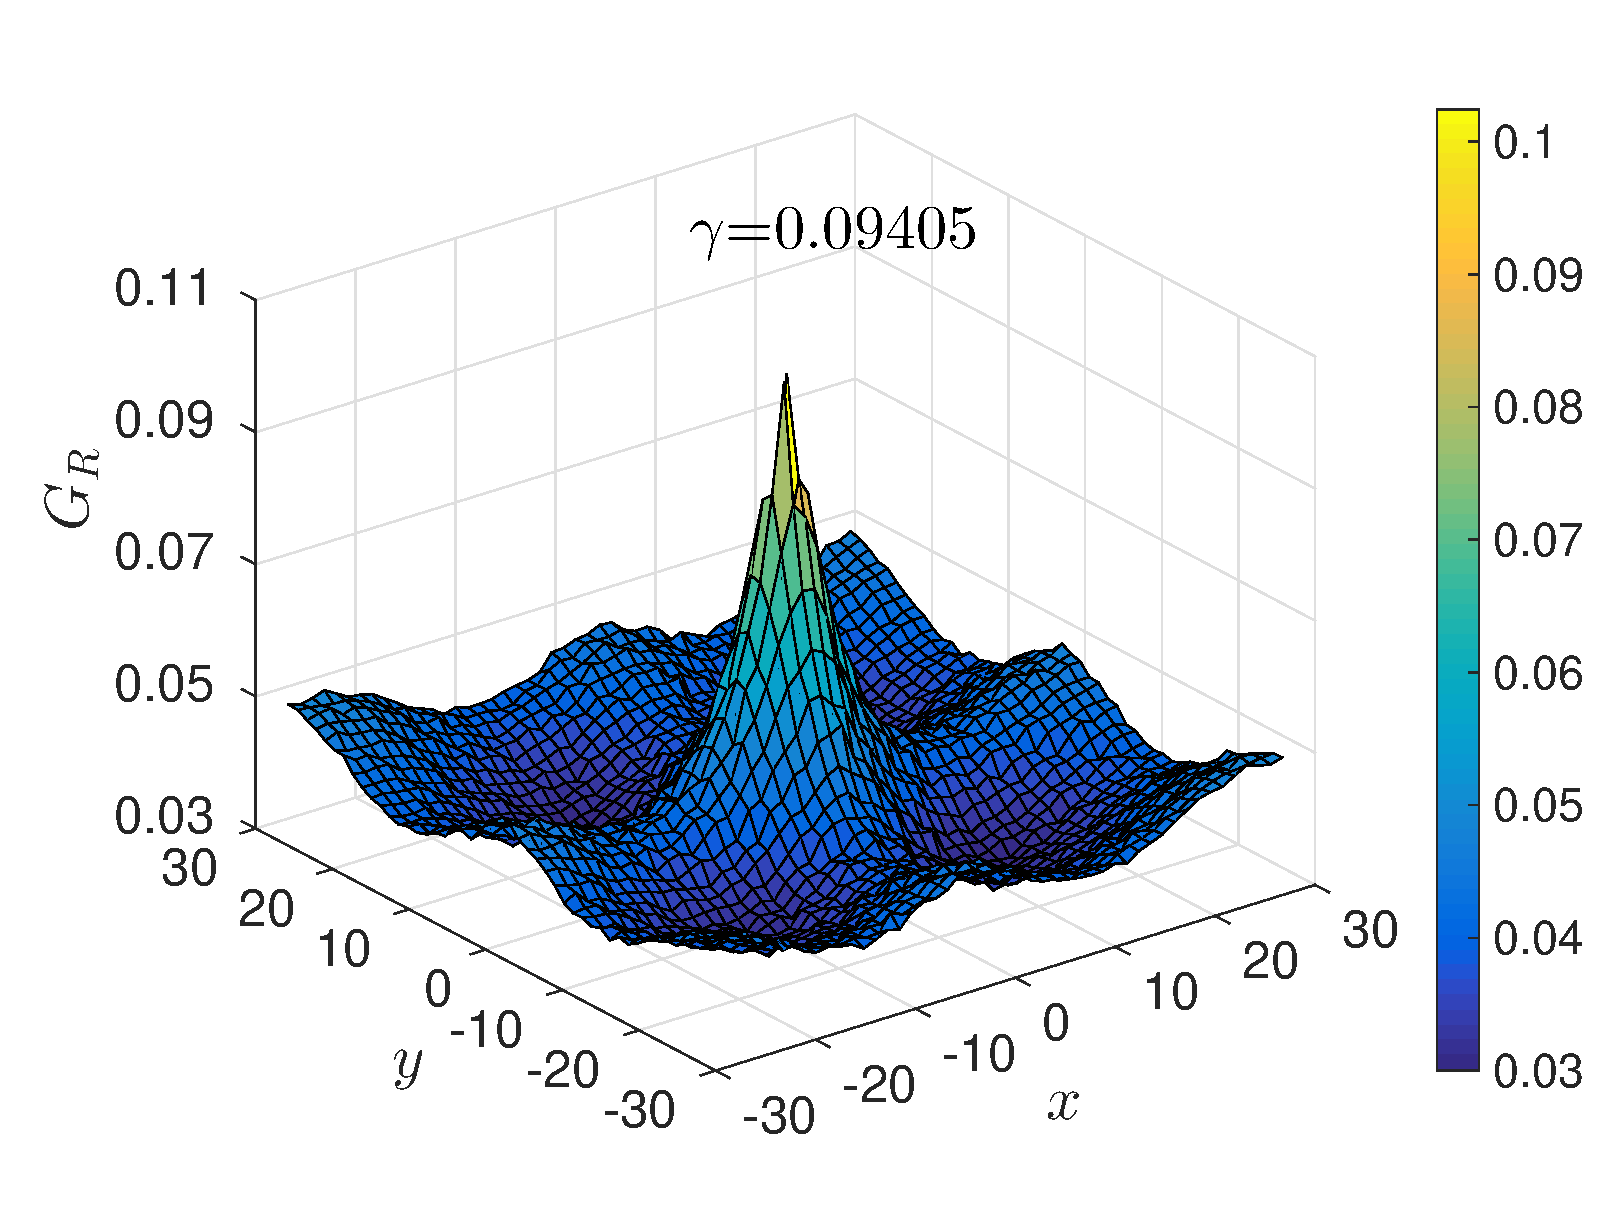
\includegraphics[width=0.3\textwidth]{spinodalSIFig2b.eps}
 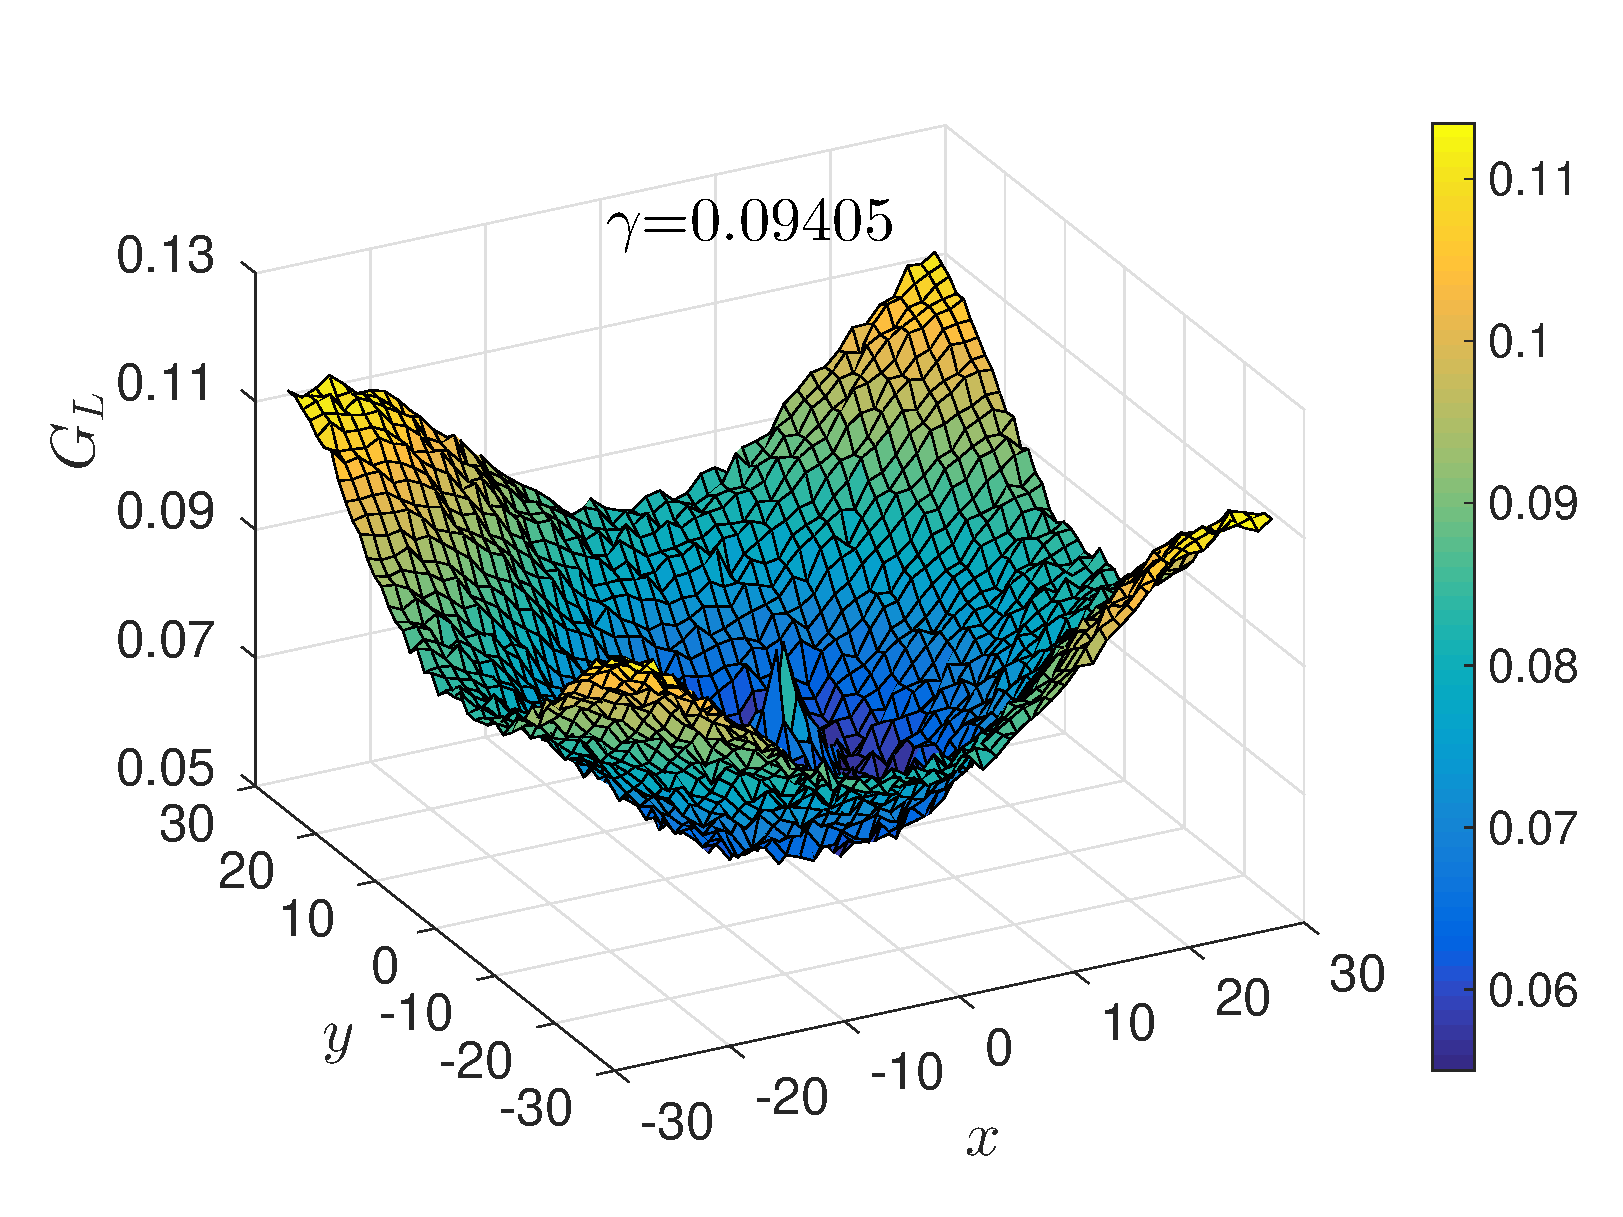
\includegraphics[width=0.3\textwidth]{spinodalSIFig2c.eps}\\
 \caption{A 3-dimensional projection of the three correlation function as a function of $x,y$.}
 \label{correlations}
 \end{figure}
%%%%%%%%%%%%%%%%%%%%%%%%%%%%%%%%%%%%%%%%%%

%%%%%%%%%%%%%%%%%%%%%%%%%%%%%%%%%%%%%%%%%%%%%%%%%%%%%%%%%%%%%%%%%%%%%%
\begin{figure}[htpb]
 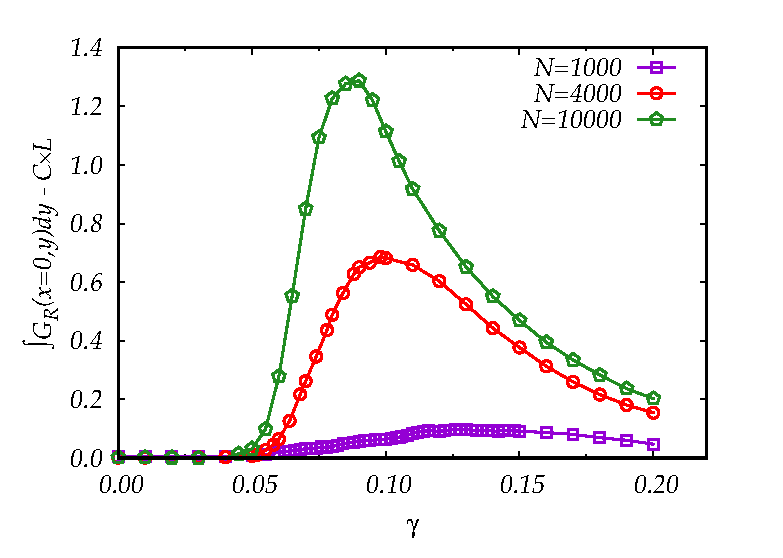
\includegraphics[width=0.45\textwidth]{spinodalSIFig3.eps}
 \caption{The difference between $\int dy\ G_R(x=0,y)$ and $C\times L$}
\label{Ceffect}
\end{figure}
%%%%%%%%%%%%%%%%%%%%%%%%%%%%%%%%%%%%%%%%%%%%%%%%%%%%%%%%%%%%%%

An interesting observation concerns the constant $C$ used in the fit Eq. 10 in the paper. This constant
is also sensitive to the approach of the criticality, cf. the lower panel in Fig.3 in the paper. One could worry
that integrating this constant over $y$ could contribute to the divergence of the susceptibilities. In fact
the rise in $C$ near the spinodal point goes down with the system size and its contribution to the integral
is reduced as well, as can be seen in Fig.~\ref{Ceffect} which presents the integral $\int dy G_R(x=0,y)$ from
which $C\times L$ is subtracted.
The conclusion is that indeed the contribution of $C$ goes down also when integrated over the system
size, showing that the main contribution to the divergence of the susceptibility is from the divergence
of the correlation length.

Finally we need to discuss the fitting procedure for the correlation function $G_R(x=0,y)$. In Fig.~\ref{full}
we show the full results for this correlation function for all the available values of $\gamma$ and for two larger systems sizes at our disposal. One sees that the exponents decay that is used for the fit is only
reliable up to the minima of the functions. The reason for the upward trend is the periodic boundary condition that reflects the correlations. To eliminate this spurious effect we presented in the paper the fit
up to the minimum in the function. One should note however that the distance to the minimum increases
with the system size, presumably diverging in the thermodynamic limit. Thus the fit up to the minimum
allows a faithful estimate of the correlation length $\xi$.
\begin{figure}[htb]
 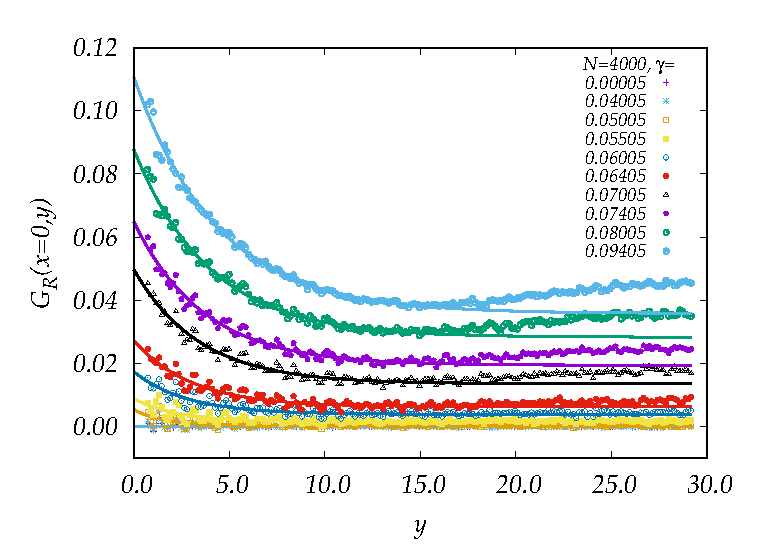
\includegraphics[width=0.45\textwidth]{spinodalSIFig4a.eps}
 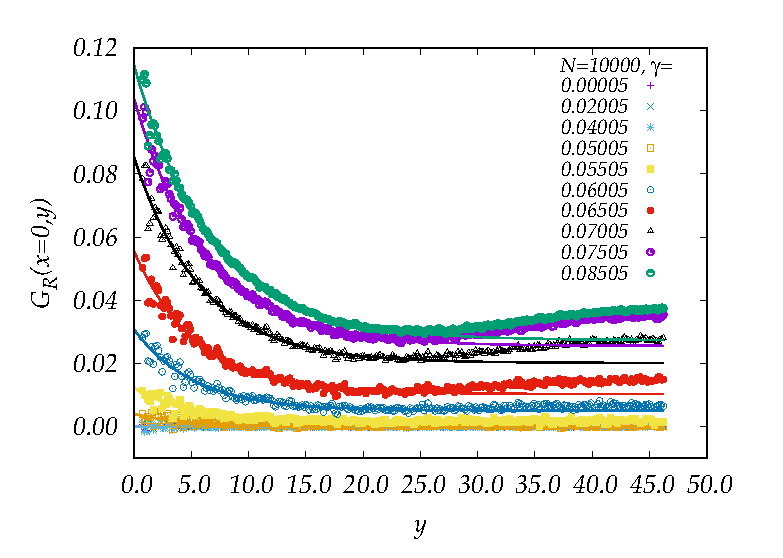
\includegraphics[width=0.45\textwidth]{spinodalSIFig4b.eps}
\caption{The full $y$ dependence of $G_R(x=0,y)$. The region fitted by Eq.~(10) in the paper
is shown. Note that the minimum in the function resides in higher values of $y$ for larger
system sizes.}
\label{full}
\end{figure}


%\bibliography{LJ}

\begin{thebibliography}{13}
\expandafter\ifx\csname natexlab\endcsname\relax\def\natexlab#1{#1}\fi
\expandafter\ifx\csname bibnamefont\endcsname\relax
  \def\bibnamefont#1{#1}\fi
\expandafter\ifx\csname bibfnamefont\endcsname\relax
  \def\bibfnamefont#1{#1}\fi
\expandafter\ifx\csname citenamefont\endcsname\relax
  \def\citenamefont#1{#1}\fi
\expandafter\ifx\csname url\endcsname\relax
  \def\url#1{\texttt{#1}}\fi
\expandafter\ifx\csname urlprefix\endcsname\relax\def\urlprefix{URL }\fi
\providecommand{\bibinfo}[2]{#2}
\providecommand{\eprint}[2][]{\url{#2}}

\bibitem[{\citenamefont{Franz and Parisi}(1995)}]{FP95}
\bibinfo{author}{\bibfnamefont{S.}~\bibnamefont{Franz}} \bibnamefont{and}
  \bibinfo{author}{\bibfnamefont{G.}~\bibnamefont{Parisi}},
  \bibinfo{journal}{J. Phys. I France} \textbf{\bibinfo{volume}{5}},
  \bibinfo{pages}{1401} (\bibinfo{year}{1995}),
  \urlprefix\url{http://dx.doi.org/10.1051/jp1:1995201}.

\bibitem[{\citenamefont{Rainone et~al.}(2015)\citenamefont{Rainone, Urbani,
  Yoshino, and Zamponi}}]{RUYZ15}
\bibinfo{author}{\bibfnamefont{C.}~\bibnamefont{Rainone}},
  \bibinfo{author}{\bibfnamefont{P.}~\bibnamefont{Urbani}},
  \bibinfo{author}{\bibfnamefont{H.}~\bibnamefont{Yoshino}}, \bibnamefont{and}
  \bibinfo{author}{\bibfnamefont{F.}~\bibnamefont{Zamponi}},
  \bibinfo{journal}{Phys. Rev. Lett.} \textbf{\bibinfo{volume}{114}},
  \bibinfo{pages}{015701} (\bibinfo{year}{2015}),
  \urlprefix\url{http://link.aps.org/doi/10.1103/PhysRevLett.114.015701}.

\bibitem[{\citenamefont{Jaiswal et~al.}(2016)\citenamefont{Jaiswal, Procaccia,
  Rainone, and Singh}}]{JPRS16}
\bibinfo{author}{\bibfnamefont{P.~K.} \bibnamefont{Jaiswal}},
  \bibinfo{author}{\bibfnamefont{I.}~\bibnamefont{Procaccia}},
  \bibinfo{author}{\bibfnamefont{C.}~\bibnamefont{Rainone}}, \bibnamefont{and}
  \bibinfo{author}{\bibfnamefont{M.}~\bibnamefont{Singh}},
  \bibinfo{journal}{Phys. Rev. Lett.} \textbf{\bibinfo{volume}{116}},
  \bibinfo{pages}{085501} (\bibinfo{year}{2016}),
  \urlprefix\url{http://link.aps.org/doi/10.1103/PhysRevLett.116.085501}.

\bibitem[{\citenamefont{Rainone and Urbani}(2016)}]{RU16}
\bibinfo{author}{\bibfnamefont{C.}~\bibnamefont{Rainone}} \bibnamefont{and}
  \bibinfo{author}{\bibfnamefont{P.}~\bibnamefont{Urbani}},
  \bibinfo{journal}{Journal of Statistical Mechanics: Theory and Experiment}
  \textbf{\bibinfo{volume}{2016}}, \bibinfo{pages}{053302}
  (\bibinfo{year}{2016}),
  \urlprefix\url{http://stacks.iop.org/1742-5468/2016/i=5/a=053302}.

\bibitem[{\citenamefont{Kurchan et~al.}(2012)\citenamefont{Kurchan, Parisi, and
  Zamponi}}]{KPZ12}
\bibinfo{author}{\bibfnamefont{J.}~\bibnamefont{Kurchan}},
  \bibinfo{author}{\bibfnamefont{G.}~\bibnamefont{Parisi}}, \bibnamefont{and}
  \bibinfo{author}{\bibfnamefont{F.}~\bibnamefont{Zamponi}},
  \bibinfo{journal}{Journal of Statistical Mechanics: Theory and Experiment}
  \textbf{\bibinfo{volume}{2012}}, \bibinfo{pages}{P10012}
  (\bibinfo{year}{2012}),
  \urlprefix\url{http://stacks.iop.org/1742-5468/2012/i=10/a=P10012}.

\bibitem[{\citenamefont{Bender and Orszag}(1999)}]{BenderAdvancedMethods}
\bibinfo{author}{\bibfnamefont{C.~M.} \bibnamefont{Bender}} \bibnamefont{and}
  \bibinfo{author}{\bibfnamefont{S.~A.} \bibnamefont{Orszag}},
  \emph{\bibinfo{title}{Advanced Mathematical Methods for Scientists and
  Engineers I}} (\bibinfo{publisher}{Springer Science \& Business Media},
  \bibinfo{year}{1999}).

\bibitem[{\citenamefont{Rainone}(2014)}]{replicanotes}
\bibinfo{author}{\bibfnamefont{C.}~\bibnamefont{Rainone}},
  \bibinfo{journal}{arXiv preprint arXiv:1411.3941}  (\bibinfo{year}{2014}).

\bibitem[{\citenamefont{Crisanti and Sommers}(1992)}]{CS92}
\bibinfo{author}{\bibfnamefont{A.}~\bibnamefont{Crisanti}} \bibnamefont{and}
  \bibinfo{author}{\bibfnamefont{H.-J.} \bibnamefont{Sommers}},
  \bibinfo{journal}{Zeitschrift f{\"u}r Physik B}
  \textbf{\bibinfo{volume}{87}}, \bibinfo{pages}{341} (\bibinfo{year}{1992}),
  ISSN \bibinfo{issn}{0722-3277},
  \urlprefix\url{http://dx.doi.org/10.1007/BF01309287}.

\bibitem[{\citenamefont{Bray and Moore}(1979)}]{BM79}
\bibinfo{author}{\bibfnamefont{A.}~\bibnamefont{Bray}} \bibnamefont{and}
  \bibinfo{author}{\bibfnamefont{M.}~\bibnamefont{Moore}},
  \bibinfo{journal}{Journal of Physics C: Solid State Physics}
  \textbf{\bibinfo{volume}{12}}, \bibinfo{pages}{79} (\bibinfo{year}{1979}).

\bibitem[{\citenamefont{De~Dominicis et~al.}(1998)\citenamefont{De~Dominicis,
  Kondor, and Temesv{\'a}ri}}]{DK98}
\bibinfo{author}{\bibfnamefont{C.}~\bibnamefont{De~Dominicis}},
  \bibinfo{author}{\bibfnamefont{I.}~\bibnamefont{Kondor}}, \bibnamefont{and}
  \bibinfo{author}{\bibfnamefont{T.}~\bibnamefont{Temesv{\'a}ri}}, in
  \emph{\bibinfo{booktitle}{Spin glasses and random fields}}
  (\bibinfo{publisher}{World Scientific, Singapore}, \bibinfo{year}{1998}), pp.
  \bibinfo{pages}{119--160}.

\bibitem[{\citenamefont{{Zamponi}}(2010)}]{Z10}
\bibinfo{author}{\bibfnamefont{F.}~\bibnamefont{{Zamponi}}},
  \bibinfo{journal}{ArXiv e-prints}  (\bibinfo{year}{2010}),
  \eprint{1008.4844}.

\bibitem[{\citenamefont{{Urbani} and {Zamponi}}(2016)}]{UZ16}
\bibinfo{author}{\bibfnamefont{P.}~\bibnamefont{{Urbani}}} \bibnamefont{and}
  \bibinfo{author}{\bibfnamefont{F.}~\bibnamefont{{Zamponi}}},
  \bibinfo{journal}{ArXiv e-prints}  (\bibinfo{year}{2016}),
  \eprint{1610.06804}.

\bibitem[{\citenamefont{Berthier et~al.}(2016)\citenamefont{Berthier,
  Charbonneau, Jin, Parisi, Seoane, and Zamponi}}]{BCJPSZ16}
\bibinfo{author}{\bibfnamefont{L.}~\bibnamefont{Berthier}},
  \bibinfo{author}{\bibfnamefont{P.}~\bibnamefont{Charbonneau}},
  \bibinfo{author}{\bibfnamefont{Y.}~\bibnamefont{Jin}},
  \bibinfo{author}{\bibfnamefont{G.}~\bibnamefont{Parisi}},
  \bibinfo{author}{\bibfnamefont{B.}~\bibnamefont{Seoane}}, \bibnamefont{and}
  \bibinfo{author}{\bibfnamefont{F.}~\bibnamefont{Zamponi}},
  \bibinfo{journal}{Proceedings of the National Academy of Sciences}
  \textbf{\bibinfo{volume}{113}}, \bibinfo{pages}{8397} (\bibinfo{year}{2016}),
  \eprint{http://www.pnas.org/content/113/30/8397.full.pdf},
  \urlprefix\url{http://www.pnas.org/content/113/30/8397.abstract}.

\end{thebibliography}

\end{document}
